\chapter{Introducción}
\label{chap:introduccion}

\section{Contextualización}
\textit{[Describir el entorno donde se identifica la necesidad del proyecto, indicando el sector, área de aplicación y situación actual. Incluir información relevante de la entidad receptora o del contexto donde se implementará la solución.]}


\section{Estado del Arte}
\textit{[Presentar la revisión de soluciones, tecnologías, metodologías o proyectos similares relacionados con el tema del proyecto. Analizar mínimo cinco (5) trabajos provenientes de fuentes académicas, técnicas o industriales, citados según normas IEEE. Incluir comparación, ventajas, limitaciones y relación con el proyecto propuesto.]}

Ejemplo de redacción con citas IEEE: para fundamentar una propuesta tecnológica se puede citar el estado del arte en inteligencia artificial y aprendizaje profundo en \cite{vaswani2017attention,goodfellow2016deep}. Del mismo modo, para enfoques de ingeniería de software y proceso de desarrollo pueden emplearse fuentes como \cite{sommerville2016software,boehm1988spiral}.

\section{Planteamiento del Problema}
\textit{[Definir de forma clara y precisa el problema o brecha tecnológica identificada. Describir las causas que lo originan y los efectos que genera en el contexto analizado. No incluir la solución en esta sección.]}

\section{Justificación}
\textit{[Redactar un texto argumentativo que exponga la importancia del proyecto, su impacto técnico y operativo, la utilidad de la solución, los beneficiarios directos e indirectos y la factibilidad técnica y operativa de su implementación.]}

\section{Objetivos}
\subsection{Objetivo General}
\textit{[Redactar el propósito principal del proyecto, alineado con la solución propuesta e incluyendo explícitamente su implementación.]}
\subsection{Objetivos Específicos}
\textit{[Enumerar acciones concretas, medibles y verificables que permitan alcanzar el objetivo general. Los objetivos deben cubrir análisis, diseño, implementación y validación.]}

\section{Alcance del Proyecto}
\textit{[Delimitar los límites del proyecto, especificando claramente los componentes, módulos o funcionalidades que se incluyen, así como aquellos que se excluyen.]}

\section{Fundamentación Teórica}
\textit{[Desarrollar los fundamentos teóricos, conceptos, modelos y tecnologías que sustentan el proyecto. Debe estar relacionado directamente con la solución propuesta y su implementación, aplicable a software, hardware o infraestructura.]}

\subsection{Ejemplo de Figura 1}
Como ejemplo de referencia dentro del texto: en la Figura~\ref{fig:ejemplo_1} se presenta un recurso visual demostrativo que guía el formato esperado para los gráficos del documento.

\begin{figure}[htbp]
  \centering
  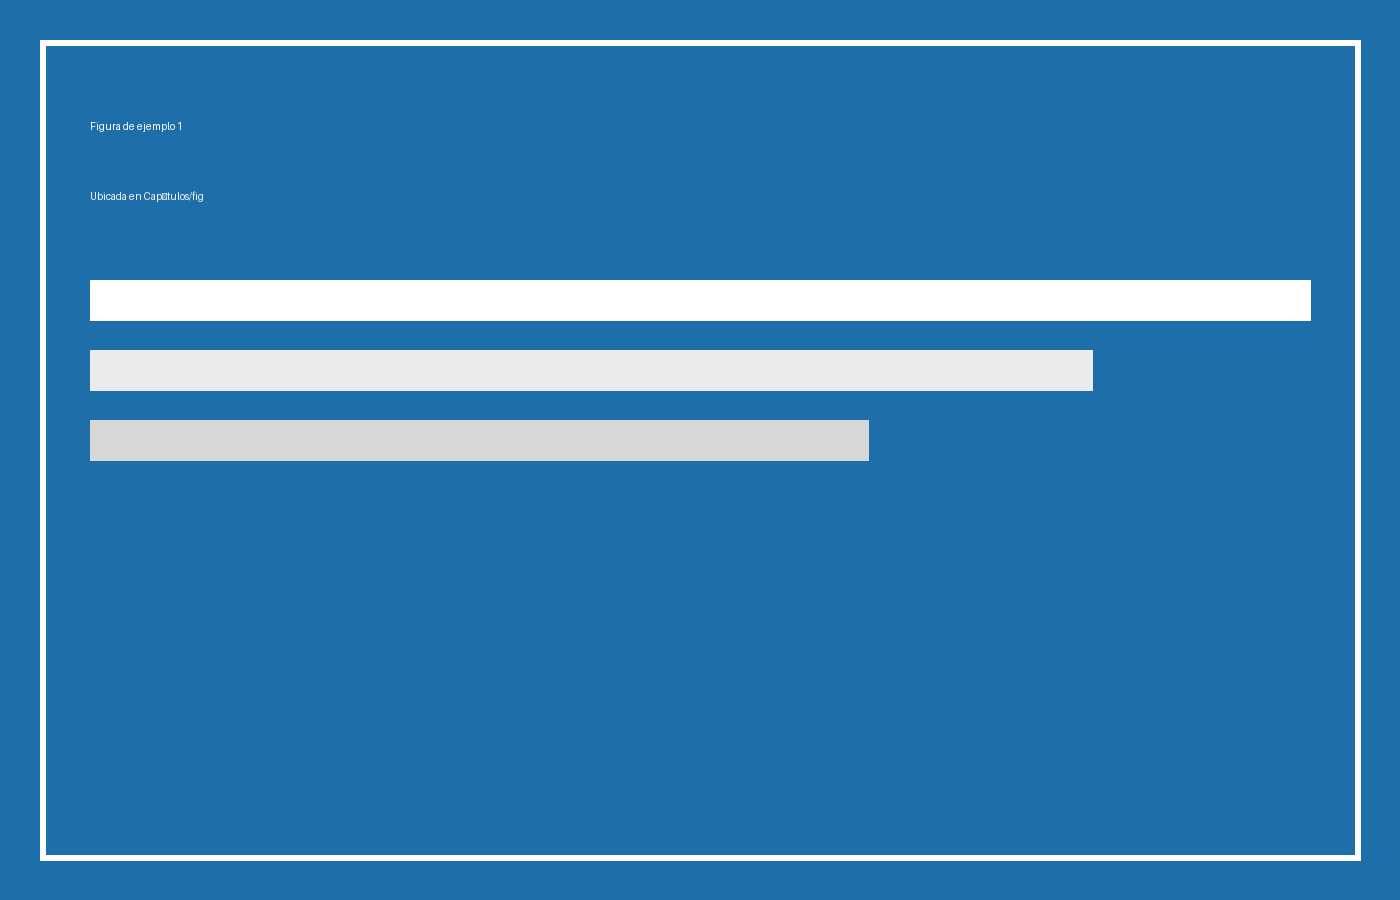
\includegraphics[width=0.80\textwidth]{Capítulos/fig/fig_ejemplo_1.png}
  \caption{Ejemplo de figura para guiar el formato de gráficos en el documento.}
  \label{fig:ejemplo_1}
\end{figure}
\elaboradopor{Estudiante}
\fuente{Elaboración propia}

\subsection{Ejemplo de Tabla 1}
Como ejemplo de referencia cruzada en párrafo: la Tabla~\ref{tab:ejemplo_1} resume indicadores base que luego pueden compararse con los resultados de implementación.

\begin{table}[htbp]
  \centering
  \caption{Ejemplo de tabla para registrar métricas iniciales del diagnóstico.}
  \label{tab:ejemplo_1}
  \begin{tabular}{|l|c|c|}
    \hline
    Indicador & Valor actual & Meta \\
    \hline
    Tiempo de respuesta (ms) & 850 & 400 \\
    \hline
    Disponibilidad (\%) & 96.2 & 99.0 \\
    \hline
    Incidencias mensuales & 14 & 6 \\
    \hline
  \end{tabular}
\end{table}
\elaboradopor{Estudiante}
\fuente{Datos de levantamiento inicial}
